\documentclass[12pt]{article}
\usepackage[english]{babel}
\usepackage[numbers]{natbib}
\usepackage{graphicx}
\usepackage{xcolor}
\usepackage{sectsty}
\usepackage{float}
\bibliographystyle{apalike}
\setcitestyle{open={[},close={]}}
\sectionfont{\color{DarkBlue}} 
\subsectionfont{\color{LightBlue}}
\subsubsectionfont{\color{LightBlue}}
\paragraphfont{\color{LightBlue}}
\subparagraphfont{\color{LightBlue}}
\begin{document}
\definecolor{DarkBlue}{HTML}{4a5a8a}
\definecolor{LightBlue}{HTML}{4f81bf}
\begin{titlepage}
\begin{flushleft}
\vspace*{1cm}
\Huge
\textbf{Cretaceous Gardens Controller}\\
\vspace{1cm}
\Huge
\textit{Requirements Definition Document}\\
\vspace{1cm}
\Large
\textit{RDD Version 1.0}\\
\vspace{5cm}
\LARGE
Team \#3\\
17 October 2019
\vfill
\Huge
\textbf{CS 460 Software Engineering}
\end{flushleft}
\end{titlepage}
\normalsize
\tableofcontents
\newpage
\section{Introduction} %Zeke
\paragraph{} \textit{//introduction}

\section{Objectives} 
\label{obj}
\paragraph{} \textit{Four objectives believed to be critical for an 
optimal implementation of a \textit{Cretaceous Gardens Controller} are identified here 
\footnote{Objectives by Anas and Siri.}.}
 
	\subsection{Safety}\label{saf}
	\paragraph{}The main objective of the CGC is to provide a safe and reliable 
	experience for the client and the end users. Whether it be electric fences 
	or autonomous vehicles, ensuring safety is of highest priority. The end user
	ought to feel completely safe as should the client whose liability depends on
	this aspect.

	\subsection{User Experience}\label{use}
	\paragraph{} In order to fully realize an amazing experience for the end user,
	the CGC must facilitate token purchases and foster intuitive and seamless interactions
	with the vehicles. 

	\subsection{Maintainability}\label{mai}
	\paragraph{} For the sake of maintainability, the state the CGC should be easily
	accessible and it should be understandable. All nodes should inherit this feature. 
	The system should also be maintainable in real-time, so it should be prepared for
	any redundancies that support this aim.
	
	\subsection{Efficiency}\label{eff}
	\paragraph{}When it comes to efficiency, the CGC will make sure that both 
	the software and hardware components are highly efficient and functional. 
	Whether we talk about self-driving cars, pay kiosks, camera system, GPS, 
	or electric fences, the CGC must be efficient in interacting with them. 
	This will be possible when all the other objectives are met.  



\section{Overall System Organization} 
\label{sys}
\paragraph{} The CGC will be centralized\footnote{System Organization 
by Anas and Siri.} and will manage all relevant components. Figure 
\ref{fig:blackbox} shows a black box diagram of the CGC. The CGC receives inputs 
from sensors, user interfaces, and emergency systems like the \textit{Global 
Alarm System} and responds through appropriate output actions as described 
below. 
\begin{figure}[H]
	\centerline{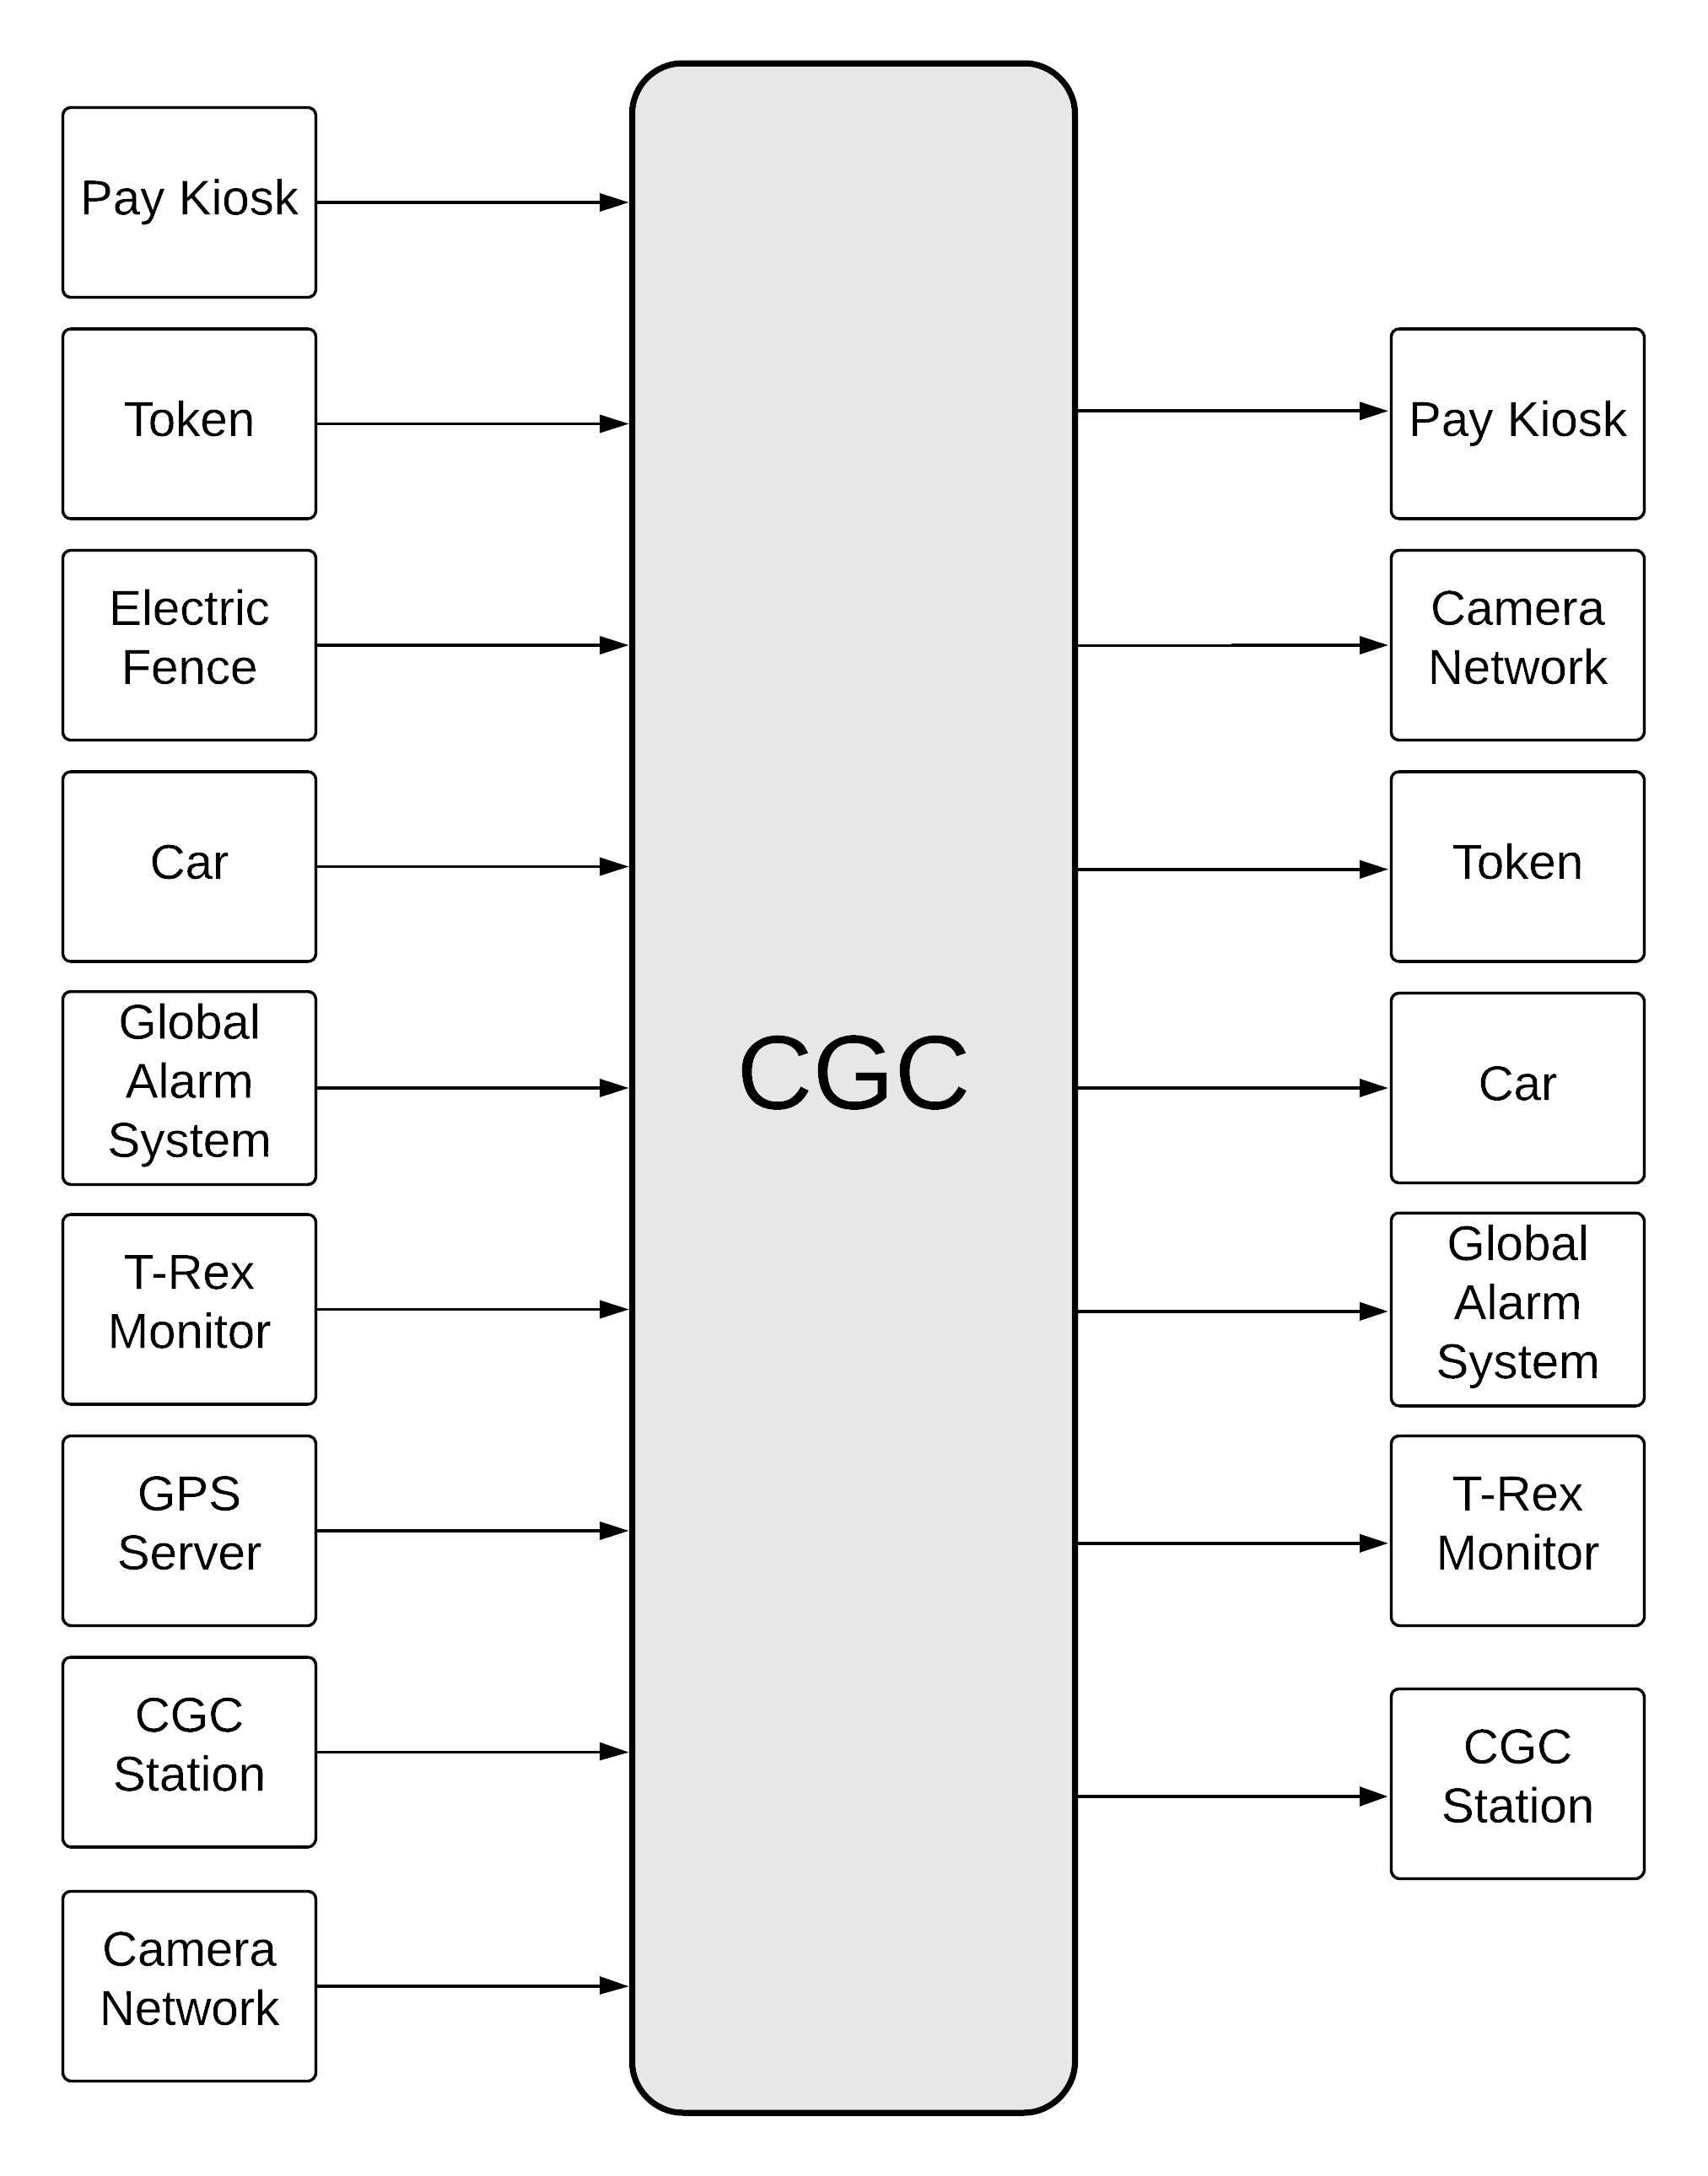
\includegraphics[scale=.20]{CGCBlackBox.png}}
	\caption{A black box of high-level inputs and outputs of the \textit{CGC}.}
	\label{fig:blackbox}
\end{figure}
\vfill
\pagebreak

\section{Interfaces}
\label{int}
\paragraph{} \textit{The interfaces are broken\footnote{Interfaces by Siri 
and Anas.} up into main systems. They may be composed of their own 
sensors but said sensors do not interface with the CGC. The following list of interfaces 
list their sensors, hardware, and features.}

	\subsection{Pay Kiosk}
	\paragraph{} \textit{The purpose of the the Pay Kiosk interface is to connect 
	the physical Pay Kiosks to the CGC. It is composed of sensors and is designed 
	to do specific feature.}
			
	\paragraph{Sensors}
	\begin{list}{}{}
		\item \textbf{Touch Screen: }used to sense user interaction. 
		\item \textbf{Credit Card: }accepts all major credit/debit cards. 
		\item \textbf{Cash Receptacle: }accepts and analyzes cash. 
	\end{list}
		
	\paragraph{Hardware}
	\begin{list}{}{}
		\item \textbf{Change Dispenser:} dispenses appropriate change to the 
		visitor buying a token.
		\item \textbf{Token Dispenser: } dispenses token with unique ID to user.
	\end{list}

	\paragraph{Features}
	\begin{list}{}{}
		\item \textbf{Token Builder:} Takes payment and the out user form and builds
		a unique token for the visitor.
		\item \textbf{Maintenance: } Enables employees to manage issues with kiosks 
		and provides machine health information. 
	\end{list}

	\subsection{Token}
	\paragraph{} \textit{The Token will act as an interface to multiple systems. 
	It will provide valuable information about the visitor and also interact with 
	the visitor. }
		
	\paragraph{Sensors}
	\begin{list}{}{}
		\item \textbf{Touch Screen: } interacts with the users. 
		\item \textbf{GPS: } senses the location of all tokens.
	\end{list}
		
	\paragraph{Hardware}
	\begin{list}{}{}
		\item \textbf{RFID: }the RFID chip will be programmed with a unique ID and 
		used for multiple purposes included access to various systems and areas.
		\item \textbf{Speaker: }the token contains speakers as hardware for alerts 
		and instructions.
	\end{list}

	\paragraph{Features}
	\begin{list}{}{}
		\item \textbf{Location/Map: }utilizes the GPS to provide location services.
	\end{list}

	\subsection{Car}
	\paragraph{} \textit{There will be an interface with all the cars. The autonomous 
	car will be built utilizing a partner. We will work closely with them to provide 
	access to specific sensors and features.}		
	
	\paragraph{Sensors}
	\begin{list}{}{}
		\item \textbf{RFID reader: }covers the proximity of the car and is used 
		to grant access and count how many tokens are currently in the car. 
		\item \textbf{Seat Weight Sensor: }used to determine if there is someone 
		sitting on the seat. 
		\item \textbf{Camera: }used by the car for autonomous driving and also 
		connects to CGC for a needed scenario. 
		\item \textbf{Microphone: }used to sense voice for use in an intercom.
	\end{list}
		
	\paragraph{Hardware}
	\begin{list}{}{}
		\item \textbf{Speaker: }used to alert guests.
		\item \textbf{Automatic Door Locks: }this will be initiated when the car 
		is determined to be moving.
		\item \textbf{Wireless networking: }for communication purposes to communicate 
		with the CGC.
	\end{list}
	
	\paragraph{Features}
	\begin{list}{}{}
		\item \textbf{Maintenance System: }allows for health checks and health status 
		communication of the car.  
	\end{list}

	\subsection{Camera Network}
	\paragraph{} \textit{The camera network interface is incharge of communicating with every camera, the redundant network links to each camera, and the DVR system that keeps recording of all cameras per retention policy. It will report on its health.}		
	
	\paragraph{Sensors}
	\begin{list}{}{}
		\item \textbf{Cameras: }records video. 
	\end{list}
		
	\paragraph{Hardware}
	\begin{list}{}{}
		\item \textbf{DVR: }stores and retains video.
		\item \textbf{Hardwire Ethernet: }used for network communication with CGC. 
	\end{list}
	
	\paragraph{Features}
	\begin{list}{}{}
		\item \textbf{Maintenance System: }allows for health checks and health status communication of the camera network.
        \item \textbf{Viewing: }ability to view any camera feed.
	\end{list}

	\subsection{Electric Fence}
	\paragraph{} \textit{The electric fence interface will ensure that the visitors are safe from the attack of T-Rex. It will provide features for maintainability, and sensing options to reduce the risk of any damage.}		
	
	\paragraph{Sensors}
	\begin{list}{}{}
		\item \textbf{Electrical Conduction Sensor: }senses for electricity going through electric fence. It has the ability to trigger when there is no electricity. 
	\end{list}
		
	\paragraph{Hardware}
	\begin{list}{}{}
		\item \textbf{Electrical Fence Panels: }special kind of physical panels that allows conductance of electricity going through it.
		\item \textbf{Hardwire Ethernet: }used for network communication with CGC. 
	\end{list}
	
	\paragraph{Features}
	\begin{list}{}{}
		\item \textbf{Maintenance System: }allows for health checks and health status communication of the electric fence.
	\end{list}

	\subsection{Global Alarm System}
	\paragraph{} \textit{The global alarm system controls what gets played on a network of speakers for emergency related or informative needs.}		

	\paragraph{Hardware}
	\begin{list}{}{}
		\item \textbf{Speaker: }the global alarm system communicates with a network of PA speakers.
		\item \textbf{Hardwire Ethernet: }used for network communication with CGC. 
	\end{list}
	
	\paragraph{Features}
	\begin{list}{}{}
		\item \textbf{Maintenance System: }allows for health checks and health status communication of the Global Alarm System.  
	\end{list}


	\subsection{CGC Station}
	\paragraph{} \textit{The CGC station is a device and interface that interacts with employees. It contains a user interface to analyze and interact with the components that the CGC can communicate with or can monitor. }		
	
	\paragraph{Sensors}
	\begin{list}{}{}
		\item \textbf{Microphone: }used to pick up voice to interact on the intercom. It can also be used to send announcements out to the Global Speaker System.
		\item \textbf{Touch Screen: }used to interact with employee with a provided GUI interface.
	\end{list}
		
	\paragraph{Hardware}
	\begin{list}{}{}
		\item \textbf{Speaker: }can be used with the intercom.
		\item \textbf{Hardwire Ethernet: }used for network communication with CGC. 
	\end{list}
	
	\paragraph{Features}
	\begin{list}{}{}
		\item \textbf{Maintenance System: }This one is unique in the sense that it can communicate with all other maintenance systems and initiate system checks. 
	\end{list}

	\subsection{GPS Server}
	\paragraph{} \textit{The GPS server interface provides locations of all the active and surrounded GPS devices that it needs to interact with. }		
	
	\paragraph{Features}
	\begin{list}{}{}
		\item \textbf{Tracking: }keeps track of all GPS devices and their longitude and latitude.
        \item \textbf{Services: }third party service to provide GPS services. 
	\end{list}

\section{Capabilities}
\label{cap}
\paragraph{}\textit{The capabilities of the system are significantly expansive due to its central role
in the operation of the resort. Thus, the complexity of the system naturally leads to a description
of the broad topography of its capabilities. First is the overview of protocol-related capabilities, then
emergency-supporting capabilities, followed by capabilities that reinforce safety features, and finally an 
overview of its monitoring capabilities.\footnote {Capabilities by Matt and Zeke.}}
% the outline for a solution
	\subsection{Protocols}
	\begin{enumerate}
		\item The CGS will have a set of specified protocols for directing the network of
		autonomous vehicles. The protocols will vary among sets of vehicles. For example, a protocol for the 
		visitor vehicles will be executed in the case of an enclosure breach, another for preparation before
		arrival of visitors and after their departure (outside business hours), another for maintenance, etc.
		\item The CGS will provide configurability of processes through straightforward interactions.
		\begin{enumerate}
			\item The creation of new protocols.
			\item The addition of pre-made protocols.
			\item The removal or extraction of protocols.
			\item The modification of existing protocols.
		\end{enumerate}
		\item The CGS will allow for the simulation of any given protocol.
	\end{enumerate}
	
	\subsection{Emergency}
	\begin{enumerate}
		\item The CGC will be able to receive distress or failure signals and propagate
		through the siren and alarm network of the island. 
		\item The CGC will be able to communicate with external authorities and emergency personnel.
		\item It will also (through human intervention) be capable of disarming the alarm system after 
		the issue has been addressed.
		\item The CGC will will be able to dynamically account for new nodes in the network or for nodes that are
		taken out for whatever reason. An extension may be that nodes may be used to triangulate the location of missing
		nodes.
	\end{enumerate}

	\subsection{Safety} 
	\begin{enumerate}
		\item The CGC will allow the monitoring of every panel of the enclosure.
		\item The CGC will allow the monitoring of every camera.
		\item The CGC will reinforce power backup measures.
		\item The CGC will maintain redundant uplinks on the network(s).
		\item The CGC will command a fleet of patrol vehicles around the island.
		\item The CGC will support a maintenance mode for real-time repair of any node.
	\end{enumerate}
	
	\subsection{Monitoring}
	\begin{enumerate}
		\item The CGC will be able to track all guests at all times.
		\item The CGC will be able to track all vehicles at all times.
		\item The CGC will be able to track the location of the T.Rex at all times.
		\item The CGC will be able to process live video stream of various locations on the island.
		\item The CGC will be able to process live video stream of the enclosure.
		\item The CGC will be able to process live video stream at kiosks.
		\item The CGC will be able to perform regular or on-demand audits of the network state.
	\end{enumerate}
	
	\subsection{Financial Analysis}
	\begin{enumerate}
		\item The CGC will be able to provide financial information and basic summary statistics.
		\item The CGC will be able to identify any striking patterns of cash flow.
		\item The CGC will be able to maintain long term financial records.
	\end{enumerate}

\section{Design Constraints} %Zeke
\label{con}
%restrictions placed on the solution space
\paragraph{} \textit{//section introduction}
	\subsection{General}
	\begin{itemize}
		\item item
	\end{itemize}
	
	\subsection{Safety}
	\begin{itemize}
		\item item
	\end{itemize}

\section{Definition of Terms} %Zeke
\label{def}
\textit{Here we have some definitions to terms used in the document. This section will help clarify meanings for different areas of the document.\footnote {Definition of Terms by Siri.}}
\begin{list}{}{}
	\item \textbf{Hardwire Ethernet: }This references the latest IEEE standard for Ethernet utilizing physical cables.
	\item \textbf{GPS: }Global Positioning System 
	\item \textbf{CGC: }Cretaceous Gardens Controller 
	\item \textbf{Electrical Conduction: }the movement of electrically charged particles through a transmission medium.
	\item \textbf{DVR: }Digital Video Recorder
	\item \textbf{Token: }Purchase receipt and access key. Also device that interacts with Visitor. We use token to represent this.
\end{list}

% the basis for accurate communication
\bibliography{../../ReferenceMaterial/BibTeX/references}
% run latex, then bibtex, then quickbuild all on the tex file
\end{document}
